%% This is based on bare_conf.tex
%% V1.3
%% 2007/01/11
%% by Michael Shell
%% See:
%% http://www.michaelshell.org/
%% for current contact information.
%%
%% This is a skeleton file demonstrating the use of IEEEtran.cls
%% (requires IEEEtran.cls version 1.7 or later) with an IEEE conference paper.
%%
%% Support sites:
%% http://www.michaelshell.org/tex/ieeetran/
%% http://www.ctan.org/tex-archive/macros/latex/contrib/IEEEtran/
%% and
%% http://www.ieee.org/
%\documentclass[conference,a4paper]
\documentclass[a4paper,10pt]{article}
\usepackage{cite}
\usepackage[pdftex]{graphicx}
\usepackage[cmex10]{amsmath}
\usepackage{fixltx2e}
\usepackage{url}

\begin{document}
%
% paper title
% can use linebreaks \\ within to get better formatting as desired
\title{ESG Seminar Experiment \\ Dynamic Dataflow and Open Event Machine}

% author names and affiliations
% use a multiple column layout for up to three different
% affiliations
\author{Risto Vuorio}
%\IEEEauthorblockA{Your Association}

% make the title area
\maketitle

\begin{abstract}
\end{abstract}

\section{Introduction}
Dataflow models of computation are well suited for stream processing tasks. There are many kinds of dataflow models but in this experiment the focus is on dynamic dataflow. Dynamic dataflow models have good powers of expression. The dynamic dataflow graphs allow for conditional execution of actors, which can be used for the construction of iterations and many other logic flows in the dataflow graphs. In general the resulting graphs are not statically schedulable. The dynamic scheduling of the actors is left for the dataflow framework.~\cite{semmapaperi} In this experiment a program of which high level structure is compatible with dynamic dataflow is implemented using Open Event Machine.

\section{Experiment Construction}
OpenEM is a runtime system for concurrent programming developed by Nokia Solutions and Networks. An introduction to the OpenEM framework can be found in~\cite{dippa}. In this experiment Canny edge detection algorithm~\cite{canny} for video streams is implemented using OpenEM~\cite{openemwhite} and vlib~\cite{vlib} by Texas Instruments. The image processing and feature detection functions used in this experiment are provided in vlib. To keep things simple input and output are omitted from the experiment. The video stream is uploaded to the device memory using Code Composer Studio tools.

\subsection{Dynamic Dataflow Model}
The dynamic dataflow model corresponding to the system under study is presented in figure~\ref{fig:ddf_model}. In the dataflow graph the canny algorithm is split into two parts. The first part consists of computing the gaussian filter, the x and y gradients and the maximum values of the gradients for the input frame. The first part is computed for all frames. The first part is followed by frame dropping decision that is represented in the figure~\ref{fig:ddf_model} by the \textbf{Random Decision} and \textbf{Drop Frame} actors.

The random decision actor takes the frame number as its input and makes random decision to drop the frame. The probability of dropping the frame is dependent on the frame number and the experiment scheme. The random decision actor is followed by the second part of the canny filter. The second part consists of computation of the hysteresis thresholding and cleaning the output of data used only in the intermediate steps of the algorithm.

\begin{figure}[!h]
    \centering
        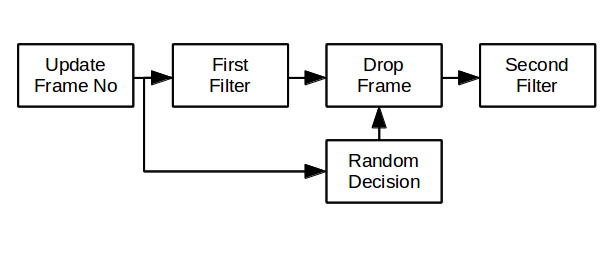
\includegraphics[width=30pc]{ddf_model.png}
        \caption{Dynamic Dataflow model corresponding to the experiment program}
        \label{fig:ddf_model}
\end{figure}

\subsection{OpenEM Implementation of the Program}
In this experiment dynamic dataflow actors are approximately mapped to OpenEM execution objects. In OpenEM there is overhead associated with the communication between the execution objects. The overhead is small compared to the computation of the filters. To keep the system under study simple as simple as possible, the number of independent actors in the OpenEM implementation of the ddf model is less than the number of ddf actors.

Frame numbers are updated in an independent execution object because the frame number is global and has to be accessed atomically. An atomic queue is connected to the frame number updating execution object. Both parts of the canny algorithm reside in their own execution objects and are connected to parallel queues. The actors constituting the random frame dropping are combined with the first part of the canny algorithm. With these modifications the number of execution objects becomes three.


\bibliographystyle{IEEEtran}
\bibliography{papers}

\end{document}

